\documentclass[a4paper,12pt]{article}
\usepackage{fixltx2e}
\usepackage{float}

\usepackage[latin2]{inputenc}
% \usepackage{huhyphn}
\usepackage[magyar]{babel}
% \newcommand{\setR}{\mathbb{R}}
% \newcommand{\setB}{\mathbb{B}}
% \newcommand{\setL}{\mathbb{L}}
% \newcommand{\setK}{\mathbb{K}}
% \newcommand{\setN}{\mathbb{N}}
\usepackage{algorithmic}

\usepackage{fancyhdr}
\usepackage{wrapfig}
% \usepackage{dottex}
\usepackage{psfrag}
\usepackage{multirow}
\usepackage{amsmath}
\usepackage{setspace}
\usepackage{graphicx,color}
% \usepackage[top=2cm, bottom=1cm, left=3cm, right=1cm]{geometry}
\usepackage[top=2.5cm, bottom=2.5cm, left=3.5cm, right=2.5cm]{geometry}
\usepackage{subfig}
% \usepackage{supertabular}
\usepackage{longtable,colortbl,tabularx,ulem}
\usepackage{hyperref}


\makeatletter
\renewcommand\paragraph{\@startsection{paragraph}{4}{0mm}%
{0.0\baselineskip}%
{0.1\baselineskip}%
{\normalfont\bfseries}%
}%

\usepackage{ktex}
% \usepackage[utf8]{inputenc}

\usepackage{amssymb}
\usepackage{textcomp}

% \linespread{1}

% % PAGE STYLE
\pagestyle{fancyplain}
\pagenumbering{arabic}
\fancyhead[CO,CE]{}
\renewcommand{\headrulewidth}{0.4pt}
\renewcommand{\footrulewidth}{0.4pt}
\fancyhead[RO,LE]{\tt{NetWorkers}
% \tiny{(r\REVISION)}
}
% \newcommand{\tailrulewidth}{0.4pt}
\fancyfoot[C]{}
% \lhead[]{TITLE}
% \rhead[]{\thepage}
% \fancyhead[LE,RO]{\thepage}
\fancyheadoffset[]{1em}

\definecolor{MyDarkBlue}{rgb}{0.85,0.85,0.85}

\usepackage{ltxtable}
% \fancyfoot[LO,RE]{\bf{ffc\_center}	\VEH }
% \rfoot{\thepage}
% \rhead{\thepage}
\usepackage{subfig}

\newcommand{\REVISION}{140M}


% \documentclass[12pt]{report}


\newcommand{\MSG}[2][]{$\overline{\mbox{\textit{#2}}}$\phantom{.}}
\newcommand{\SER}{\Gamma}

% \newcommand{\MSG}[2][]{$\overline{{{#2}}}$}
\newcommand{\SUR}{\MSG{scan\_update\_req}}
\newcommand{\SU}{\MSG{scan\_update}}
\newcommand{\SI}{\MSG{scan\_info}}
\newcommand{\LI}{\MSG{link\_info}}
\newcommand{\IL}{\MSG{interlock}}
\newcommand{\HB}{\MSG{heartbeat}}
\newcommand{\LE}{\MSG{link\_error}}
\newcommand{\MD}{\MSG{measure\_depth}}
\newcommand{\HO}{\MSG{hand\_over}}
\newcommand{\LO}{\MSG{length\_opt}}


\newcommand{\TOWER}{\widehat{tower}}
\newcommand{\SWEEP}{\widehat{sweep}}
\newcommand{\RECON}{\widehat{recon}}
\newcommand{\INIT}{\widehat{init}}
\newcommand{\CP}{\complement}
\newcommand{\LEADER}{\spadesuit}

\newcommand{\V}{\underline{v}}
\newcommand{\M}{\underline{m}}
\usepackage{rotating}
\fancyfoot[CO,CE]{\thepage}
% \fancyfoot[C]{}
% \fancyfoot[RO,RE]{\slshape 7/15/2002}


\newcommand{\HRule}{\rule{\linewidth}{0.2mm}}

\begin{document}




% \chead{}
\normalfont

\boldmath
\normalsize
\numberwithin{equation}{section} 

% \begin{center}
% \huge{networkers}\\
% % \small{Nagy Zolt�n\footnote{kirk@bteam.hu}}\\
% \small{svn\footnote{https://demeter.teteny.bme.hu/svn/networkers/trunk}r\REVISION}
% % \small{\today\\ svn\footnote{https://demeter.teteny.bme.hu/svn/networkers/trunk}r\REVISION}
% \end{center}
% 
% 
% % \begin{figure}[h!]
% % % \begin{figure}[h]
% % % \vspace{-1.5em}
% % \centering
% % \includegraphics[width=.75\textwidth]{fig/elte}
% % % \vspace{-2em}
% % % \caption{szabad mozg�si t�r}
% % % \vspace{-2em}
% % % \caption{rug�er�k }
% % % \label{fig:spring_power}
% % % \label{fig:spring_power}
% % % \end{figure}
% % \end{figure}
% 
% % \large
% 
% \newpage

% \pagestyle{empty} % Use for title page, or use
% \begin{titlepage}
% \begin{center}
% 	\begin{Huge}
% % E�tv�s Lor�nd Tudom�nyegyetem\\
% % Informatikai Kar
% 	\end{Huge}
% \end{center}
% \begin{figure}[h!]
%  \centering
% % \includegraphics[width=.55\textwidth]{fig/elte-t}
% \end{figure}
% \begin{center}
% 
% % 	\begin{Huge}
% % 	NetWorkers
% % 	\end{Huge}\\
% \vspace{16em}
% 	\begin{Large}
% 	 	TDK dolgozat
% 	\end{Large}\\\vspace{3em}
% 	\begin{normalsize}
% 	K�sz�tette: Nagy Zolt�n
% 	\end{normalsize}	
% 
% \end{center}
% % xxx
% \end{titlepage}
% \newpage


\pagestyle{empty} % Use for title page, or use
\begin{titlepage}

% \begin{multicols}{2}
%   lots of text
% \end{multicols}

% \usepackage[top=2.5cm, bottom=2.5cm, left=3.5cm, right=2.5cm]{geometry}


% \hspace{-0.1\textwidth}
\begin{minipage}{0.25\textwidth}
% \begin{flushleft} \large
% \emph{Author:}\\
% John \textsc{Smith}
% \end{flushleft}
% \begin{figure}[h!]
%  \centering
\includegraphics[width=1\textwidth]{fig/elte-t}
% \end{figure}
\end{minipage}
\begin{minipage}{0.75\textwidth}
\begin{center}
% 	\begin{large}
\textbf{
E�TV�S LOR�ND TUDOM�NYEGYETEM\\\vspace{0.5em}
\vfill
INFORMATIKAI KAR}\\\vspace{0.5em}
% 	\end{large}
\vfill
\vfill
% \vspace{2em}
% 	\begin{large}
PROGRAMOZ�SELM�LET �S\\SZOFTVERTECHNOL�GIA TANSZ�K\\
% 	\end{large}
% \emph{Author:}\\
% John \textsc{Smith}
\end{center}
\end{minipage}
% \HRule


\HRule
\vfill

% \begin{center}
% 	\begin{Huge}
% E�tv�s Lor�nd Tudom�nyegyetem\\
% Informatikai Kar
% 	\end{Huge}
% \end{center}


\begin{center}
% 	\HRule
	\begin{large}
% 	\bfseries
	\textbf{
	NetWorkers - felder�t�s �s alapvet� h�l�zat ki�p�t�se raj intelligencia seg�ts�g�vel}
	\end{large}
% 	\HRule
% 	\begin{Large}
% 	 TDK dolgozat
% 	\end{Large}\\\vspace{3em}
% 	\begin{normalsize}
% \vspace{2em}
% \begin{tabbing}
% \hspace{5em}	 \=	K�sz�tette:\hspace{2em}\=Nagy Zolt�n\\\>\>Programtervez� matematikus hallgat�\\ % (�vf: X.)\\
% % 	\>						\>kirk@rxd.hu\\
% \\
% 	\>	Konzulens(ek):\>	Dr. Istenes Zolt�n\\\>\> egyetemi docens (ELTE-PSZT)\\
% % 	\>				\>	istenes@inf.elte.hu\\
% \\
% 	\>				\>	Csikor Levente\\\>\> PhD hallgat� (BME-TMIT)\\
% % 	\>				\>	levente.csikor@tmit.bme.hu
% \end{tabbing}
% 	\end{normalsize}	

\end{center}

% \vfill
% \HRule\\
\vfill
\vfill


\begin{minipage}{.5\textwidth}
\begin{tabbing}
\hspace{1em}\=\=\\Konzulens(ek):\\
\>\>Dr. Istenes Zolt�n\\
\>\> egyetemi docens (ELTE-PSZT)\\
\>\>Csikor Levente\\
\>\> PhD hallgat� (BME-TMIT)\\
\end{tabbing}
\vfill
\end{minipage}
\begin{minipage}{.5\textwidth}
\begin{tabbing}
\hspace{1em}\=\=\\K�sz�tette:\\
\>\>Nagy Zolt�n (NAZHAET)\\
\>\>nappali tagozat\\
\>\>programtervez� matematikus hallgat�\\
\end{tabbing}
\vspace{2em}
\end{minipage}





\vfill
\begin{center}

Budapest, 2011.

\end{center}
% xxx
\end{titlepage}
\newpage
\begin{titlepage}

temabejelento helye

\end{titlepage}
\newpage

\large
\linespread{1.2}

\tableofcontents
\newpage
\listoffigures

\linespread{1.5}
\normalsize
\newpage
% \setcounter{page}{1}
\pagestyle{fancy} % No headers, just page numbers

\input{parts/20_intro}
\input{parts/30_problem}

\section{Networkers algoritmus}

�gy pr�b�ltam megoldani a feladatot, hogy a kialakul� algoritmus tov�bb\-fejleszt\-het� lehessen. Az egyik t�voli c�l, hogy a h�l�zat ki�p�t�s�ben r�sztvev� networkerek esetleges meghib�sod�si hib�ival szembe tudjon majd sz�llni. Ennek a c�lkit�z�snek el�r�s�hez az egyes networkerek auton�m egys�gekk�nt �n�ll� d�nt�seket hoznak �s rajk�nt pr�b�lj�k megoldani egy�tt a probl�m�t - ez a hossz� t�v� c�l megk�nny�ti, de sok helyen megnehez�ti az algoritmus kidolgoz�s�t.

% Az algoritmus megtervez�sekor els�dlegesen a raj intelligencia bevon�sa volt a c�l, ugyanis el�fordulhat, az ir�ny�t�s megk�t�s�t�l val� szabadul�s a m�k�d�sben sokat seg�thet - ez�ltal robosztusabb� v�lhat a rendszer, mivel a legfontosabb az egyes elemek szoros �sszetart�sa a k�z�s c�l el�r�se �rdek�ben.

% \HEAD
% Minden igyekezet ellen�re az algoritmus v�g�l annyira sok kicsi �p�t�k�b�l �p�lt fel hogy nem f�rne el k�nyelmesen egy oldalon. Ez�rt az �ttekinthet�s�g megtart�sa miatt minden egyes r�szt k�l�n-k�l�n vizsg�lunk meg.

\subsection{�ttekint�s}

Miel�tt m�g m�lyebben sz� lenne a konkr�t megold� algoritmusr�l, el�sz�r fontos, hogy az olvas� egy v�zlatos k�pet kapjon r�la �ltal�noss�gban.

Az algoritmus t�bb szerepk�rben tekint az egyes networkerekre, a k�\-l�n\-b�\-z� szerepk�rt bet�lt� networkerek egy�ttm�k�dve seg�tik egym�st. Az egyes networkerek a szerep�k szerint m�s-m�s c�llal cselekszenek:

% \sout{Minden egyes networker t�bb feladat ell�t�s�ra k�pes az hogy �ppen hogyan viselkedik az �llapot�t�l f�gg.}

\xparagraph{P�szt�z�:}
Az algoritmus indul�s�t megnehez�ti az egy pontb�l val� indul�s. A kezdeti zs�folt helyzetet a p�szt�z�k oldj�k fel egy form�ci�val, melyr�l a \ref{c_sweep} fejezetben lesz sz�.
A p�szt�z�k feladata megsz�ntetni azt, hogy egy-egy networker l�t�t�vols�g�ban ne legyen t�l sok t�rsuk.
% \sout{Az algoritmus indul�sakor felvett �llapot a z�rzavar elker�l�se �rdek�ben. Az algoritmus indul�sakor ha azonnal keres�k jelennek meg akkor a $2$-es elemnek nem l�tezik vezet�je, de minden m�s keres� sz�m�ra a r��p�tett l�nc megfelel a szab�lyoknak. De a $2$ csak akkor v�lik hasznos felder�t�v�, ha az $1$-es toronyt�l �zenetet kap, hogy az m�r egy torony; ennek pedig $\frac{1}{n}$ a val�sz�n�s�ge.}

\xparagraph{Felder�t�k:} Feladatuk, hogy l�ncokba fejl�dve �j klienspontokat kapcsoljanak az �p�l� h�\-l�\-zat\-hoz. A felder�t�k m�k�d�s�r�l a \ref{c_recon} fejezetben lesz sz�.

\xparagraph{Torony:} A toronyk�nt viselked� robotok a h�l�zat infrastrukt�r�j�t biztos�tj�k. Jelent�sen nem v�ltoztatj�k meg a helyzet�ket, javar�szt a h�l�zat �letben\-tart�s�hoz sz�ks�ges robotsz�mot pr�b�lj�k cs�kkenteni.

\xparagraph{Tov�bbi mindig teljes�l� tulajdons�gok:}
\begin{itemize}
	\item mindig l�tezik legal�bb egy torony �llapot� robot, s ez�ltal mindig l�tezik az a gr�f, melyet a torony �llapot� robotok fesz�tenek.
	\item	nem szakadhat le egy �gens sem
\end{itemize}

\hspace{-1em}Minden k�rben h�rom f� m�veletet v�geznek el az egyes �gensek:
\begin{enumerate}
	\item	�zenetek feldolgoz�sa
	\item	d�nt�s az �llapotv�lt�sr�l
	\item	elmozdul�s
\end{enumerate}


\newpage

\subsubsection{�zenetek}

Az egyes robotok a bet�lt�tt szerep�knek megfelel�en k�l�nb�z� �zeneteket hasz\-n�l\-nak az egym�ssal t�rt�n� kommunik�ci�hoz, melyek t�pust�l f�ggetlen�l a k�vetkez� id�pillanatra �rnek el a felad�t�l a c�mzettig.

% Az algoritmus t�bb t�pus� �zenetet haszn�l a kommunik�ci�khoz - ezen �zenetek mindig csak a k�vetkez� id�pillanatra �rnek el a c�mzetthez.

Az �zeneteket egys�gesen d�lt bet�kkel �s fel�lvonal�ssal jel�l�m.

\begin{itemize}
	\item{\SI :}	az algoritmus tartalmaz egy v�letlenen alapul� �zenetk�ld�st, mely lehet�v� teszi a fogad� sz�m�ra, hogy tudom�st szerezzen valamely szomsz�dja azonos�t�j�r�l �s �llapot�r�l.\\
	\item{\IL :}
		K�t �gens k�z�tti kommunik�ci�s �l kialak�t�s�hoz sz�k\-s�\-ges �zenet. Az ilyen �lek mindk�t v�gpontja torony szerepet t�lt be legk�s�bb ezen �zenet fogad�sa ut�n.
% amennyiben sz�ks�ges hogy k�t �gens k�z�tt egy kommunik�ci�s �l j�jj�n l�tre azt ezzel az �zenettel jelzik egym�snak.

% 	A sz�banforg� �l a felad� ~ k�ld� k�z�tti.\\

	\item{\SUR :}	a felder�t� robotoknak mindig van egy ``ismer�se '', akihez m�rten a l�ncform�ci�t fel szeretn� venni - de ehhez sz�ks�ge van a form�ci� ir�nyvektor�ra, ami id�k�zben v�ltozhat, ez�rt minden k�rben megk�rdezi.
	\\
	\item{\SU :}	a felder�t�sben r�sztvev� �gensek minden k�rben t�\-j�\-koz\-tat\-j�k a szomsz�djukat a jelenleg alkalmazott keres�si ir�nyr�l - ezt az �zenetet csak v�laszk�nt kaphatja egy robot a \SUR -re.\\
	\item{\LE :}
		Az el�bbi �zenet hat�s�ra kialak�tott kommunik�ci�s �lek meg\-sz�n\-te\-t�\-s�\-hez sz�ks�ges.
% ha egy �gens �gygondolja hogy egy kommunik�ci�s �lre m�r nincs sz�ks�g ezzel az �zenettel jelzi az �l megsz�ntet�s�t a szomsz�dnak.

	Ahogy az \IL �zenetn�l, itt is a felad�-k�ld� �lr�l t�rt�nik nyilatkoz�s.

	\item{\MD :}	a gr�f maxim�lis �tm�r�j�t m�ri

	\item{\LO :}	be�gyaz�sra ker�lt egy v�letlen t�bbforr�s� gr�f\-m�ly\-s�g\-m�\-r�s - ezt az �zenett�pust k�l�n fejezetben t�rgyalom

\end{itemize}


\newpage

% \subsection{Klienspontok}
\subsubsection{Elv�r�sok a klienspontokt�l}

Mivel az algoritmusnak megvan a maga menete, ez�rt a kli\-ens\-pon\-tok\-t�l is megk�vetel egy bizonyos szint� protokollt,
mely a k�vetkez�k�pp fogalmaz\-hat� meg:
amennyiben egy �sszek�t�vel nem rendelkez� klienspont \SI \phantom{x} �zenetet kap, azt egy \IL �zenettel nyugt�znia kell.
% hogyha egy \SI �zenet kap akkor ha m�g nincs �sszek�t�je akkor nyugt�znia kell a k�r�st egy
%  \IL �zenet visszak�ld�s�vel.
Emellett, ha m�r l�tezik �sszek�t�je, de az t�volabb van, mint a k�rdez�, akkor azt a megfelel� �zenetekkel cser�lje le a k�zelebb l�v�re.


% \XFIG{.33}{dia/problem_2pw}{xy}{Tervezett felt�lt�s}
% \XFIG{.33}{dia/problem_2px}{xy}{Tervezett felt�lt�s}


\subsubsection{Indul�s}
Minden egys�g keres�($\RECON$) �s tov�bb�t�($\TOWER$), ezt az aktu�lis �llapota ha\-t�\-roz\-za meg.
Mindemellett egy kezdeti($\INIT$) �llapottal, valamint egy sz�t\-sz�r�\-d�si f�\-zis\-sal($\SWEEP$) is rendelkeznek.

A kezdeti �llapotban minden �gens a sz�tsz�r�d�sra k�sz�l fel, kiv�ve az $1$-es sorsz�m� robotot, amely azonnal toronny� v�lik.

Az $1$-es �gens toronny� v�l�sa k�telez�, mert az algoritmus csak a m�r megl�v� gr�fot b�v�ti az �sszef�gg�s�g biztos meg�rz�se �rdek�ben.


% \subsubsection{Az algor

% \subsubsection{Az algoritmus kialak�t�s�hoz felhaszn�lt


% _____





\input{parts/50_sweep}
\input{parts/60_recon}
\subsection{Gr�fcs�csok - $\TOWER$}
\label{c_tower}

Azon felder�t�k, melyek egy �j �rt�kes klienspontot tal�lnak, tornyokk� v�l\-nak. Ebben az �llapotban az �gens feladata n�h�ny szomsz�dj�val
t�rt�n�
 kapcsolattart�s (oly m�don, hogy azoknak ne ker�lj�n hat�sugar�n k�v�lre), va\-la\-mint az arra t�ved� felder�t�knek val� �tmutat�s.

Minden torony �llapotban l�v� robot rendelkezik szomsz�dai halmaz�val ($K$). Ez a halmaz mindig tartalmaz legal�bb egy elemet - amennyiben pontosan egy elemet tartalmaz, akkor az �gens megpr�b�l lev�lni, �s felder�t�k�nt tov�bb folytatni a kutat�st egy �j klienspont ut�n.

Ha egy keres� �j cs�csot tal�l, akkor ennek hat�s�ra egy \IL �zenet v�gigfut a keres�l�ncon, am�g el nem �ri a m�r megl�v� gr�f perem�t. Hab�r ezut�n az �j klienspont hozz� van kapcsolva a m�r l�tez� h�l�zathoz, de k�nnyen megeshet, hogy a keres�k el�g �gyetlen�l tal�lt�k meg (p�ld�ul a kellet�n�l s�r�bben �lltak fel). Ez�rt
mindenk�pp j� lenne kihaszn�lni a tornyok eset�ben is azok mobilit�si k�pess�g�t, �s megpr�b�lni cs�kkenteni a h�l�zat fenntart�s�hoz sz�ks�ges �gensek sz�m�t, �s �gy egy�ttal n�velni a keres�k sz�m�t.

% A tornyok feladat�nak �sszetetts�ge indokolta hogy olyan 


Olyan m�dszerre van sz�ks�g, mely seg�ts�g�vel a tornyok elmozdulhatnak, de meg kell tudni tartaniuk a kapcsolataikat a szomsz�dos tornyokkal. 
Az irodalomban t�bb helyen tal�lkoztam a rug�er�kkel (\cite{1208965},\cite{SPR}), mely egy nagyon egyszer� �s j�l haszn�lhat� m�dszer.

\subsubsection{Rug�er�k}


K�zelebbi vizsg�l�d�s sor�n n�ha anom�li�k l�ptek fel, mely annak volt k�\-sz�n\-he\-t�, hogy rug�er�k alkalmaz�sa eset�n a \ref{springs}. �br�n l�that� probl�m�val kell szembes�lni. Ugyanis a rug�er�k k�pesek egy adott ir�nyba t�ls�gosan is nagy er�t kifejteni, amennyiben t�bb pont csoportosul egy m�sikkal szemben.


\XFIG{.4}{dia/spring_power}{springs}{A rug�er�kkel val� probl�ma szeml�ltet�se }




% \begin{figure}[h]
% \vspace{-1em}
% 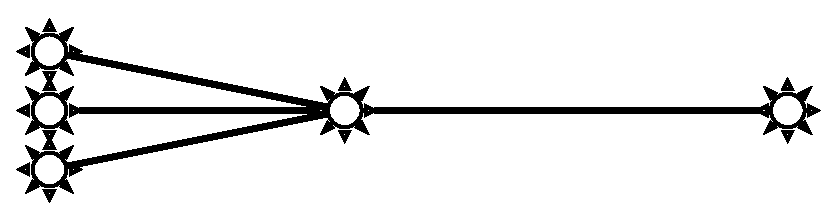
\includegraphics[width=.45\textwidth]{dia/spring_power}
% \vspace{-1em}
% \caption{rug�er�k }
% \label{fig:spring_power}
% \end{figure}

% Ez�rt a rug�er�k lecser�l�sekor a k�vetkez� c�loknak kellett megfelelnie az 
A helyettes�t�s�re egy olyan m�dszert kerestem, ami megtartja a rug�er� pozit�v tulajdons�gait, de kev�sb� �rz�keny az \ref{springs}. �br�n l�that� csoportosul�sra. Egy olyan k�z�p�rt�ket kellett keresni, ami a rug�er�h�z hasonl�an valamilyen energiaminimum-pont fel� tend�l, viszont nem annyira �rz�keny arra, hogy a pontok milyen form�ban helyezkednek el.
Ez a probl�ma hasonl�t egy pontcsoport legjobb bels� pontj�nak meghat�roz�s�hoz.

\FEL{Adott} $n$ pont a s�kon $p_i \in \setR^2$, c�l meghat�rozni egy olyan pontot, mely k�zel azonos t�vols�gra van a pontokt�l azok csoportosul�s�t�l f�ggetlen�l.

\MEGJ	A s�lypont el�g k�zel �ll a probl�ma megold�s�hoz, csak a pont\-cso\-por\-tot kell j�l megv�lasztani.


% \vspace{1em}
\vspace{1em}


Az alap�tlet ($gavg$) az, hogy �gy szeretn�m s�lyozni, hogy a pontok sz�ma ne sz�m�tson annyira. Ez�rt a pontok �ltal kifesz�tett soksz�g �leinek �sszes pontja alapj�n �llap�tom meg a k�z�ppontot.

\xparagraph{gavg}
Vegy�k a pontokat valamilyen k�r�lj�r�si ir�ny szerint rendezve, p�ld�ul az �tlagolt pontb�l n�zve (ez az amit megadnak a $0$-ban elt�n� rug�er�k ), ezut�n konstru�lhatunk olyan $f_i(x)$ f�ggv�nyeket, melyek az $i.$ �l pontjait v�gigl�togatj�k. $f_i(\lambda)=x_{i-1} * \lambda + (1-\lambda)*x_i$.
Ahova szeretn�nk eljutni az a k�vetkez�: �tlagoljuk az alakzatunk �leinek pontjainak vektorait, ezt �gy tehetj�k meg, hogy  az $f$ f�ggv�ny�nk minden pontj�t megs�lyozzuk az ottani deriv�lttal.
\begin{equation}
\frac{\int_0^1 \|f'\| f}{\int_0^1 \|f'\|}
\end{equation}

N�mi fejteget�s ut�n a k�vetkez� egyszer�s�tett k�plet ad�dik:

\begin{equation}
 gavg(P) = \frac{\sum_{i=1}^n \vec{x_i} * ( || x_{i-1} - x_i||_2 + || x_{i} - x_{i+1}||_2 ) }{2  \sum_1^n || x_{i} - x_{i-1}||_2 }
\end{equation}


\MEGJ{Az egyszer�s�g kedv��rt az $x_0$ pont megegyezik az $x_n$-el.}
\MEGJ{A $P=\{ x_1,x_2 ... x_n \}$ ponthalmaz, p�ld�ul az �ramutat� j�r�sa szerint rendezve.}

% Az �gy meghat�rozott pont jelent�sen cs�kkentette a cs�nya 


\XFIG{.3}{dia/freedist}{fdist}{Szabad mozg�si t�r (fdist)}

F�ggetlen�l az alkalmazott k�z�ppont meghat�roz�si m�dszert�l, az adott k�z�p\-pont m�g nem biztos�t tervezett t�vols�got a kiindul�pontokt�l. Ez�rt sz�ks�g van a k�vetkez� seg�t� f�ggv�nyre:
\xparagraph{A szabadt�vols�g (fdist)} Azt adja meg, hogy mekkora az a t�vols�g, amit az adott pont m�g a t�vols�gi korl�tok megs�rt�se n�lk�l elmozdulhat (\ref{fdist}. �bra):

% $$ fdist(q,P,r) = \max(0, (\max_{p\inP}( ||p-q||_2 )-r )/r) $$
\begin{equation}
  fdist(q,P,r) = \max(0,\frac{r-\max_{p\in P} d(p,q)}{r})
\end{equation}


% Ez a k�rd�s nagyon hasonl�t a k�vetkez�h�z:

% \xparagraph{Egy nem kipr�b�lt alternat�va} lehetne a k�vetkez� is:
% 	s�lyozzuk a pontokat a norm�l �tlagb�l l�tsz�si sz�g�k szerint, vagy az aktu�lis pontb�l val� l�tszatuk alapj�n.




% \subsection{Gr�fcs�csok - $\TOWER$}
% % a m�r be�llt tornyok feladatai:
% % \begin{itemize}
% % 	\item	a gr�f k�rmentes�t�se, melyhez seg�ts�get ny�jt majd a vezet� �ltal kiadott id�nk�nti sz�vdobban�s, ha egy elem kiv�lik mert a jelenl�te sz�ks�gtelenn� v�lt akkor $\RECON$ �llapotba v�lt
% % 	\item	minimaliz�lniuk kell a gr�fhoz sz�ks�ges elemek sz�m�t,\\
% % 		minden torony a k�r�l�tte elhelyezked� tornyok k�z� akar �llni.
% % 	\item	a kommunik�ci�s pont meletti tornyok m�r�csomagokat adnak ki, mely kezdetben $1$-et majd minden toronyon val� �thalad�skor egyel n�vel�dik.
% % 	\item	a heartbeat-nek egyedi azonos�t�ja van melyet minden robot elt�rol amikor megkapja,
% % 		ha m�sodszor is megkapja akkor kiv�lik a h�l�zatb�l.
% % \end{itemize}
% 
% % \begin{wrapfigure}{r}{0.15\textwidth}
% % \vspace{-2em}
% % \psfrag{IC}[lt][lt]{\tiny{\IL}}
% % \psfrag{LE}[lb][lb]{\tiny{\LE}}
% % \psfrag{A}[cc][cc]{\tiny{A}}
% % \psfrag{B}[cc][cc]{\tiny{B}}
% % \psfrag{C}[cc][cc]{\tiny{C}}
% % % \psfrag{IC}[lt][lt]{\tiny{\IL}}
% % % \psfrag{LE}[lb][lb]{\tiny{\LE}}
% % 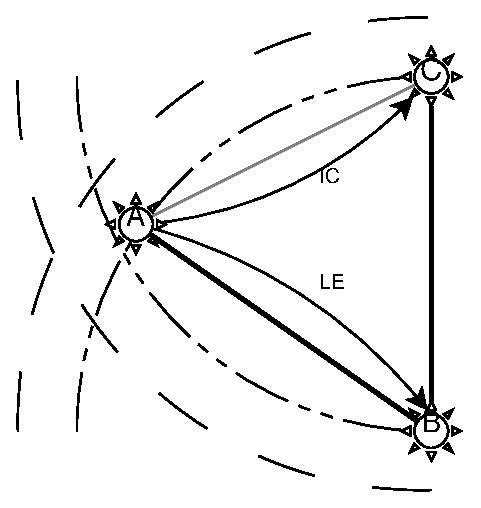
\includegraphics[width=.15\textwidth]{dia/three_towers}
% % \end{wrapfigure}
% % 
% % \xparagraph{H�rom torony probl�ma:}
% % \sout{
% % 	ha t�l k�zel ker�l egym�shoz h�rom torony akkor nem teljesen egy�rtelm� hogy mit is kellene tenni, ugyanis egy id� ut�n ha a tornyok v�lthatnak szomsz�dokat akkor el��llhatnak olyan  esetek hogy egy toronyra m�r nincs t�bb� sz�ks�g - s �jra keres�sbe kezdhet.\\
% % A torony v�lt�st a \SI �zenet hat�s�ra fogj�k ellen�rizni a tornyok:\\
% % Az \SI-b�l kider�l hogy egy toronyr�l van sz�, s �gy az fogad� torony tudja ellen�rizni hogy �t-e szeretne cser�lni egy kapcsolatot.\\
% % El�fordulhat hogy $A$ �s $C$ egyszerre szeretne v�ltani ami �ltal egyszerre k�lden�nek \LE-t $B$ ir�ny�ba, s egy ilyen esem�ny ut�n a gr�fban egyel cs�kkenne az akt�v �lek sz�ma, aminek hat�s�ra t�bb komponensre eshetne sz�t, ez�rt a v�lt�st csak az a torony v�gezheti el akinek kissebb a sorozatsz�ma.\\
% % ILYEN MAR NINCS
% % }


A fenti k�t �tlet seg�ts�g�vel kifesz�tik a gr�fot az �gensek �s a t�vols�gokat egyenletesen elosztj�k, �gy ahogy rug�er�k eset�ben t�rt�nt volna.

Viszont ennek mell�khat�sa, hogy k�t �gens k�z�tti t�vols�g nagyon kicsiv� is v�lhat, ez�rt sz�ks�ges egy m�sik m�dszer is, melyek felv�ltva alkalmaz�s�val a tervezett t�vols�gra ker�lnek a cs�csok egym�st�l.

\xparagraph{Optimaliz�ci�s f�zisok}

A gr�f kifesz�t�se k�t alapvet� f�zisb�l �ll:
\begin{enumerate}
 \item A tornyok az el�bb bemutatott rug�er�szer� dolgot felhaszn�lva megkeresik az energiaminimum-szintj�ket �s egyenletes t�vols�gra ker�lnek egym�st�l.
 \item	A gr�f m�lys�gm�r�s�b�l ismertt� v�lik az a szomsz�d, mely legink�bb a gr�f belseje fele van.
	Amennyiben ehhez a cs�cshoz k�zelebb ker�l az �gens, abban az esetben a h�l�zat sz�leit fesz�ti ki.
\end{enumerate}


% \newpage
% \XFIG{0.7}{dia/tower_stage_opt}{tso}
\begin{figure}[h!]
% \begin{figure}[h]
% \vspace{-1.5em}
\centering
\psfrag{KX}[lb][lb]{$\hat{k}$}
\psfrag{K1}[rt][rt]{$k_1$}
\psfrag{K2}[lt][lt]{$k_2$}
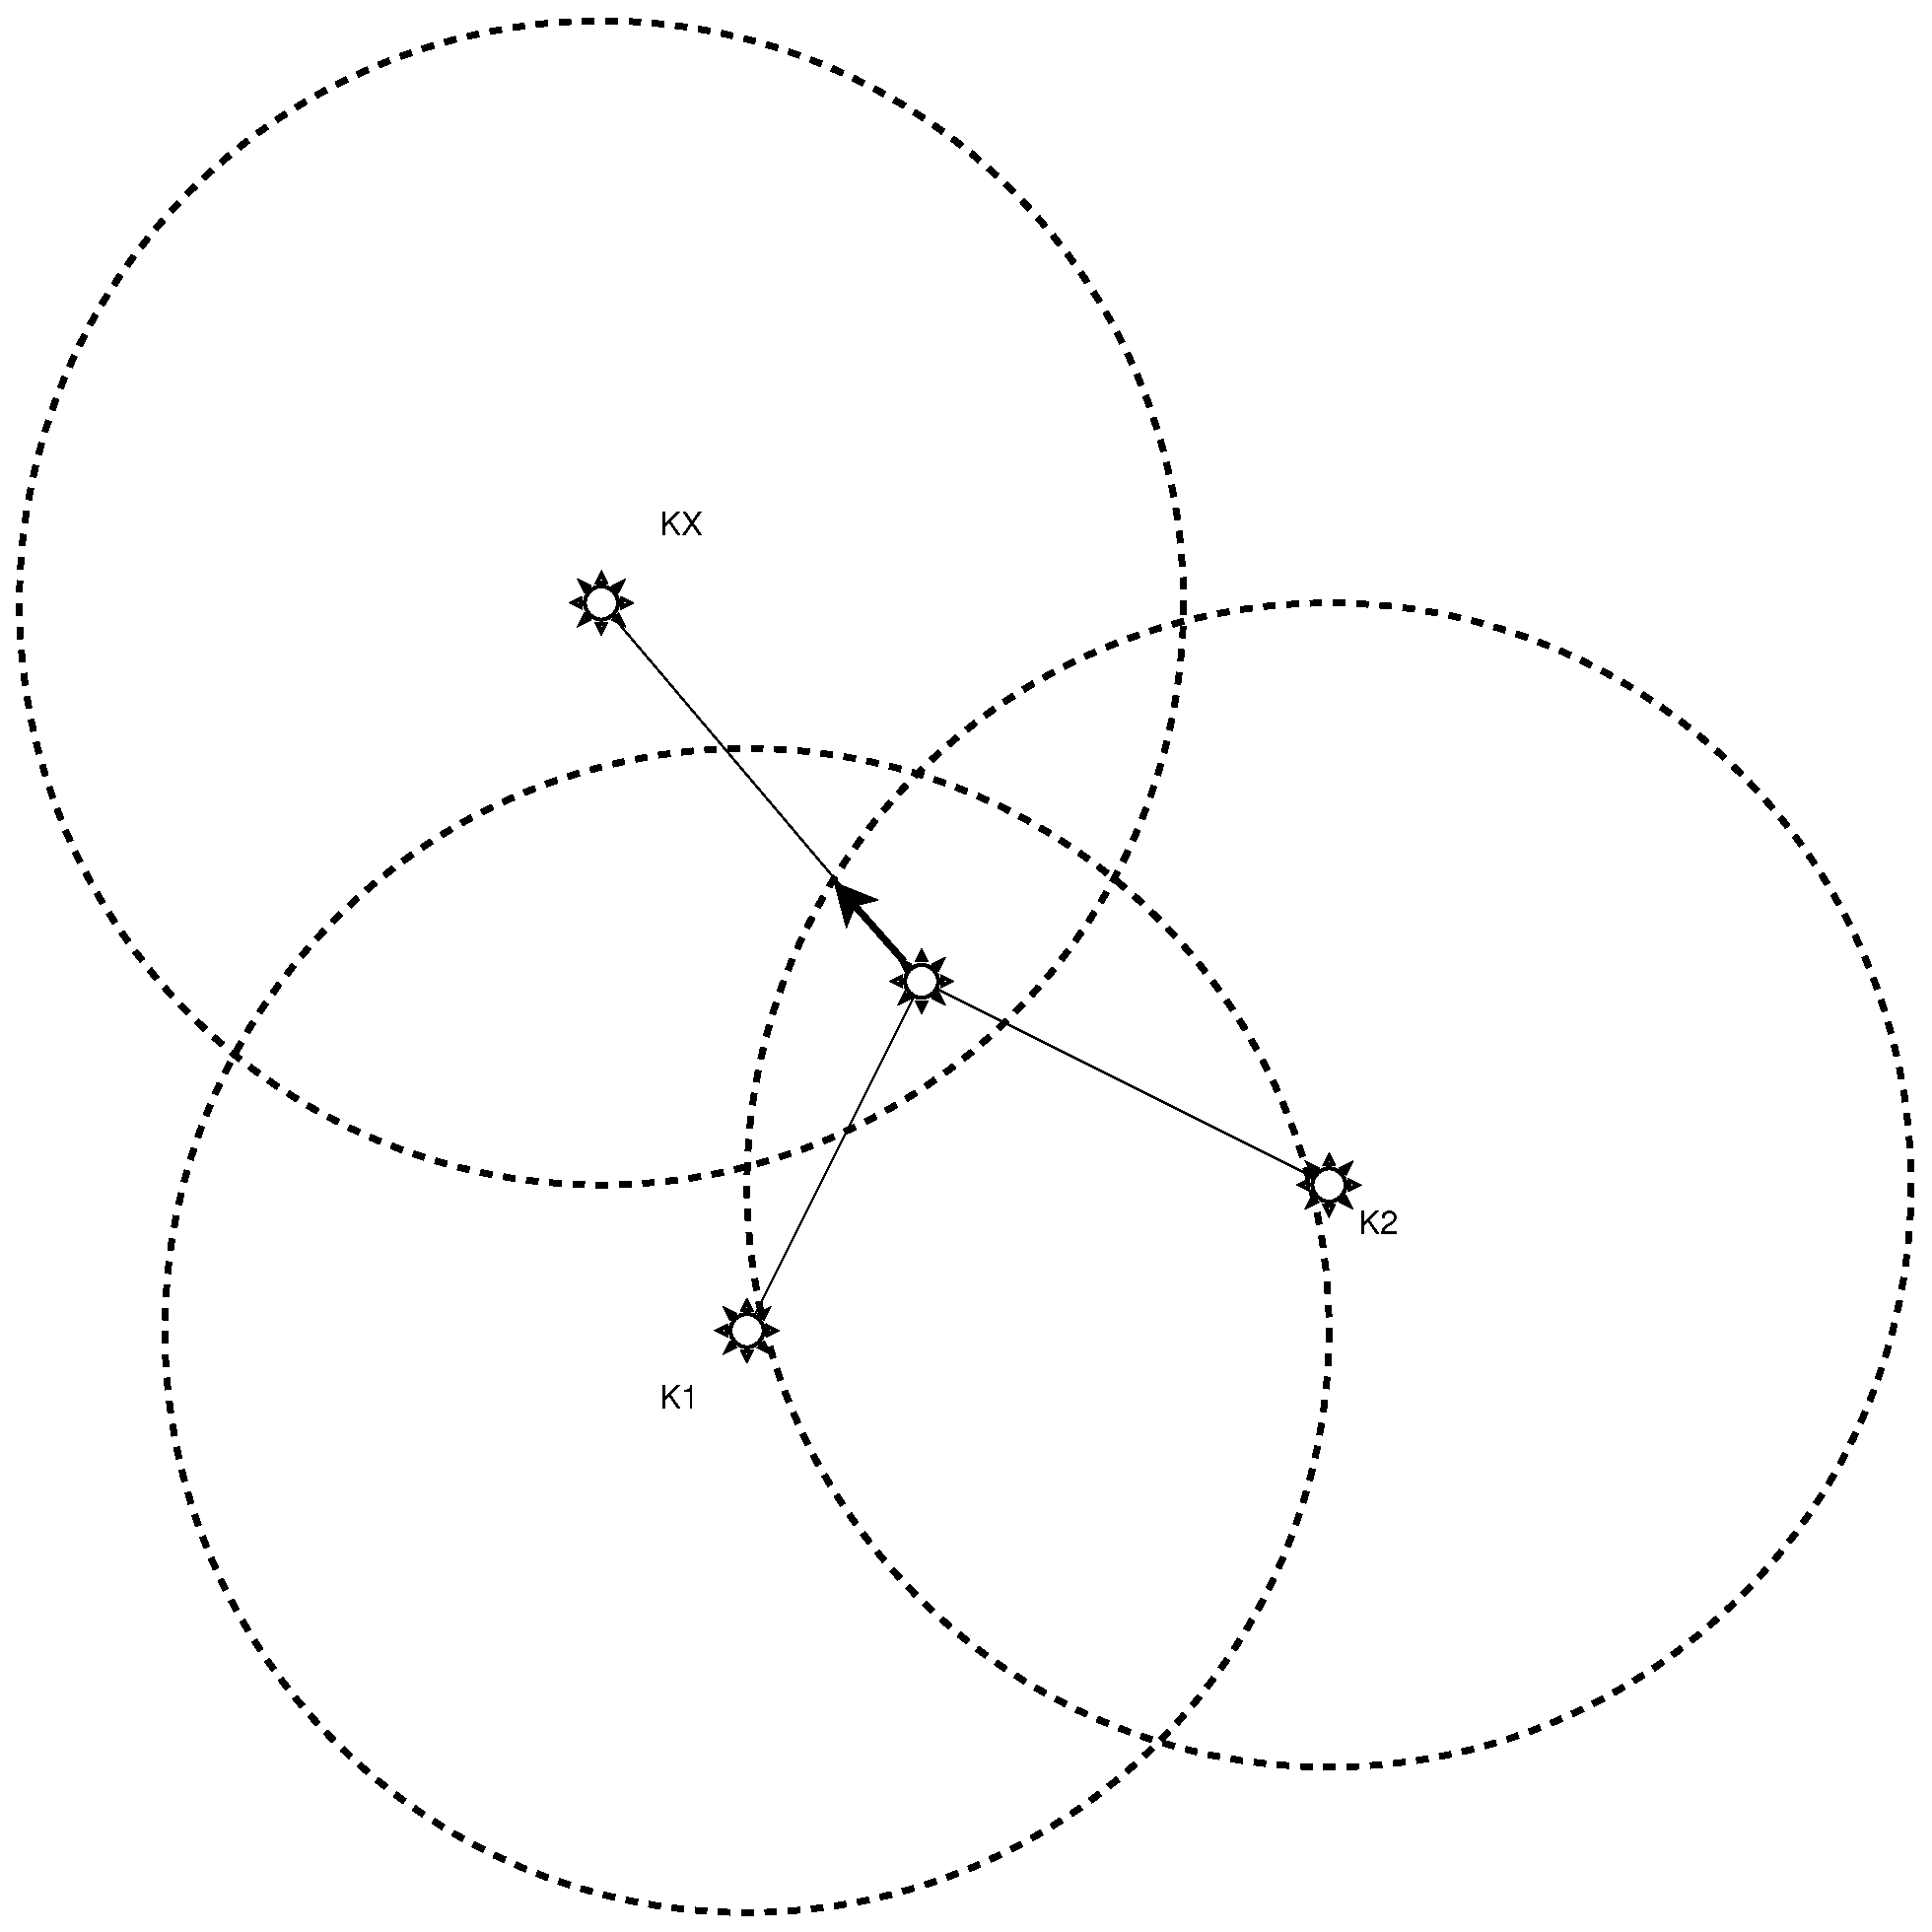
\includegraphics[trim=50mm 50mm 50mm 50mm,clip,width=.7\textwidth]{dia/tower_stage_opt}
% \vspace{-2em}



\caption{A $\hat{k}$ ir�ny�ba val� ell�p�s}
% \vspace{-2em}
% \caption{rug�er�k }
% \label{fig:spring_power}
\label{tso}
% \end{figure}
\end{figure}

A \ref{tso}. �br�n l�that� egy torony, melynek a szomsz�dai $\hat{k},k_1$ �s $k_2$.
A m�lys�gi m�r�sb�l ismert, hogy a $\hat{k}$ szomsz�dj�n �t �rhet� el a h�l�zat nagyobb r�sze. Az �gens ebben az esetben a $\hat{k},k_1$ �s $k_2$ �ltal megengedett maxim�lis elmozul�si hat�rok k�z�tt a $\hat{k}$ szomsz�d ir�ny�ba maxim�lisan l�p el, �gy r�k�nyszer�ti a $k_1$ �s $k_2$ cs�csokat, hogy m�gjobban megfesz�ts�k saj�t szomsz�daikat. Sok l�p�sen kereszt�l alkalmazva a m�dszert minden cs�cs a tervezett t�vols�gba ker�l egym�st�l.

A gr�f optimaliz�l�s�nak m�sodik f�zis�ban minden torony �r�ti az optimaliz�l� halmazt($O$).
Akik kommunik�ci�s pont mellett �llnak, felveszik azt az $O$ halmazba, �s elk�ldik minden szomsz�djuknak a m�lys�g�ket. Innent�l minden cs�cs hasonl�k�nt tesz, de bev�rja, hogy $d(v)-1$ darab optimaliz�ci�s csomagot kapjon, miel�tt tov�bbk�lden� azt, meghat�rozva ezzel a fa pontbeli �tm�r�j�t.

\newpage



\subsubsection{A h�l�zatot reprezent�l� gr�f}

A torony szerepet bet�lt� networkerek egy f�t pr�b�lnak meg kifesz�teni a klienspontok k�z�. Ahhoz, hogy a tornyok k�pesek legyenek cs�kkenteni a h�l�zat fenntart�s�hoz sz�ks�ges robotok sz�m�t, ezt a gr�fot kell megvizsg�lniuk �gy, hogy az egyes networkerek alapvet� tulajdons�gait megismerhess�k ennek a gr�fnak.


% A ki�p�l� h�l�zat alapj�ul szolg�l� gr�f m�dos�t�s�hoz egy pillanatra az eg�szet kell megvizsg�lni, hogy abb�l lok�lisan felhaszn�lhat� �tleteket nyerj�nk.
% A tornyok �ltal haszn�lt �zenetek egy r�sze a gr�f bizonyos helyi vagy glob�lis tulajdons�gair�l ad inform�ci�t.

\xparagraph{�tm�r�m�r�s}

Nagyon sokat el�rul egy �gens sz�m�ra, ha ismeri, hogy az egyes szomsz�dai mekkora �tm�r�j� r�sz�t k�pezik a teljes gr�fnak. Ezen inform�ci� birtok�ban k�pesek lesznek megfesz�teni a gr�fot, �s ez�ltal cs�kkenteni annak fenn\-tart\-�\-s�\-hoz sz�ks�ges �gensek sz�m�t.

\DEF{Gr�f �tm�r�je:}	egy gr�f �tm�r�je $k$, amennyiben b�rmely k�t pontja k�z�tt l�tezik egy legfeljebb $k$ hossz� �t.

% Gheorghe Antonoiu �s Pradip K. Srimani \cite{SELF_STAB_MST}  �nstabiliz�l� fesz�t�fa algoritmusa nagyon hasznos �r�snak bizonyult. Az alkalmazott v�ltozat kis modos�t�sokkal ker�lt be�p�t�sre



A gr�f �tm�r�j�t a k�vetkez� p�rhuzamos algoritmus(\cite{PA}) seg�ts�g�vel m�r\-het\-j�k le($K$ a szomsz�dok halmaza, $O$ egy kezdetben �res halmaz, valamint $d=0$)
\begin{enumerate}
	\item
		amennyiben $|O|=|K|-1$
		elk�ldi $d$-t a $t=O \char`\\ K$ elemnek �s a $3$ f�zisba l�p
	\item
		v�rja, hogy valamelyik szomsz�dj�t�l $s$ egy $d'$ m�r�st kapjon\\
		$d=\max(d,d'+1)$\\
		$O=O\Union \{s\}$\\
		ugr�s az $1$ pontra
% 		v�rja hogy 
% 		$O=\{\}$\\
% 		amennyiben a cs�cs foksz�ma $1$ elk�ldi az egyetlen szomsz�dj�nak hogy a k�ls� sug�r n�la $0$
	\item 
		v�rja, hogy az egyetlen szomsz�dj�t�l ($t=O \char`\\ K$), akinek elk�ldte a saj�t m�lys�g�t, �zenetet kapjon $d'$ m�r�ssel \\
		ekkor a gr�f �tm�r�je: $d'+1+d$\\
		Ahhoz, hogy mindenki rendelkezzen ezzel az inform�ci�val, m�g tov�bb kell k�ldenie a $d'+1$-et minden az $O$ halmazban felsorolt szomsz�dj�nak.
\end{enumerate}

A tornyok algoritmusa tartalmazza a fenti m�dszert, valamint az $O$ halmazt m�g arra is felhaszn�lja, hogy annak ismeret�ben tiszt�ban van vele az �gens, hogy a gr�f nagyr�sze a $t$ cs�cs ir�ny�ban van, ez�rt ahhoz az elemhez megy k�zelebb - �gy a h�lozat peremvid�k�n maxim�lis t�vols�gba ker�lhetnek az �gensek.
% remek!

\subsubsection{T�bb forr�s� m�lys�gm�r�s}



A gr�f �tm�r�j�nek ismerete sokat seg�t, de sokszor el�fordulhatnak  feleslegesen kialakult bek�t�utak, melyek helyett sokkal r�videbbekre is lehet�s�g lenne.

Az ilyen jelleg� hib�kon jav�tani lehet, ha l�tezik egy olyan r�videbb m�g fel nem haszn�lt �l, mely bev�tel�vel egy m�sik �l v�lik a legnehezebb�.
De ehhez sz�ks�ges valamilyen m�don s�lyozni:
a k�t szomsz�ddal rendelkez� tornyok igaz�b�l nem tekinthet�ek bels� pontoknak, s�t legink�bb s�lyok, mivel ha kevesebbel is megoldhat�, akkor azt valamilyen m�don figyelembe kell venni. 

Amennyiben v�letlenszer�en v�lasztan�nk egy cs�csot, �s att�l m�rn�nk minden cs�cs t�\-vol\-s�\-g�t, akkor lehets�ges jav�tani az ilyen jelleg� hib�kon - azonban ha a gr�f m�r viszonylag nagy, akkor ezen cs�cs kiv�laszt�sa csak a k�rnyezet�ben l�v� hib�kon tud seg�teni a t�volabbiakat nem fedi fel. Ez�rt egyszerre t�bb cs�csot v�lasztok.
A gr�fot tulajdonk�ppen egyszerre t�bb sz�nnel sz�nezem ki, ez�ltal megn�velve az es�ly�t annak, hogy ezen hib�k felfedhet�ek legyenek.

% Ahhoz, hogy az ilyeneken jav�t�s t�rt�nhessen viszont nem elegend� csup�n a gr�f m�lys�g�re hagyatkozni ez�rt a gr�fot t�bb sz�nnel fogom kiszinezni.
V�lasszunk n�h�ny cs�csot v�letlenszer�en, �s m�rj�k meg minden cs�cs t�\-vol\-s�\-g�t ezekt�l a cs�csokt�l, valamint t�telezz�k fel, hogy l�tezik egy olyan �sszekapcsolhat� jav�t��l, amivel k�nny�thet�nk a gr�fon.

\XFIGG{0.95}{dia/depth_opt}{fig:comm1}{M�lys�gi jav�t�s}{
	\psfrag{CP}[cc][cc]{klienspontok}
	\psfrag{TOWER}[cc][cc]{tornyok}
	\psfrag{RECON}[rc][rc]{felder�t�k}
	\psfrag{G}[cc][cc]{$G$}
}
% \begin{figure}[h]
% \vspace{-1em}
% 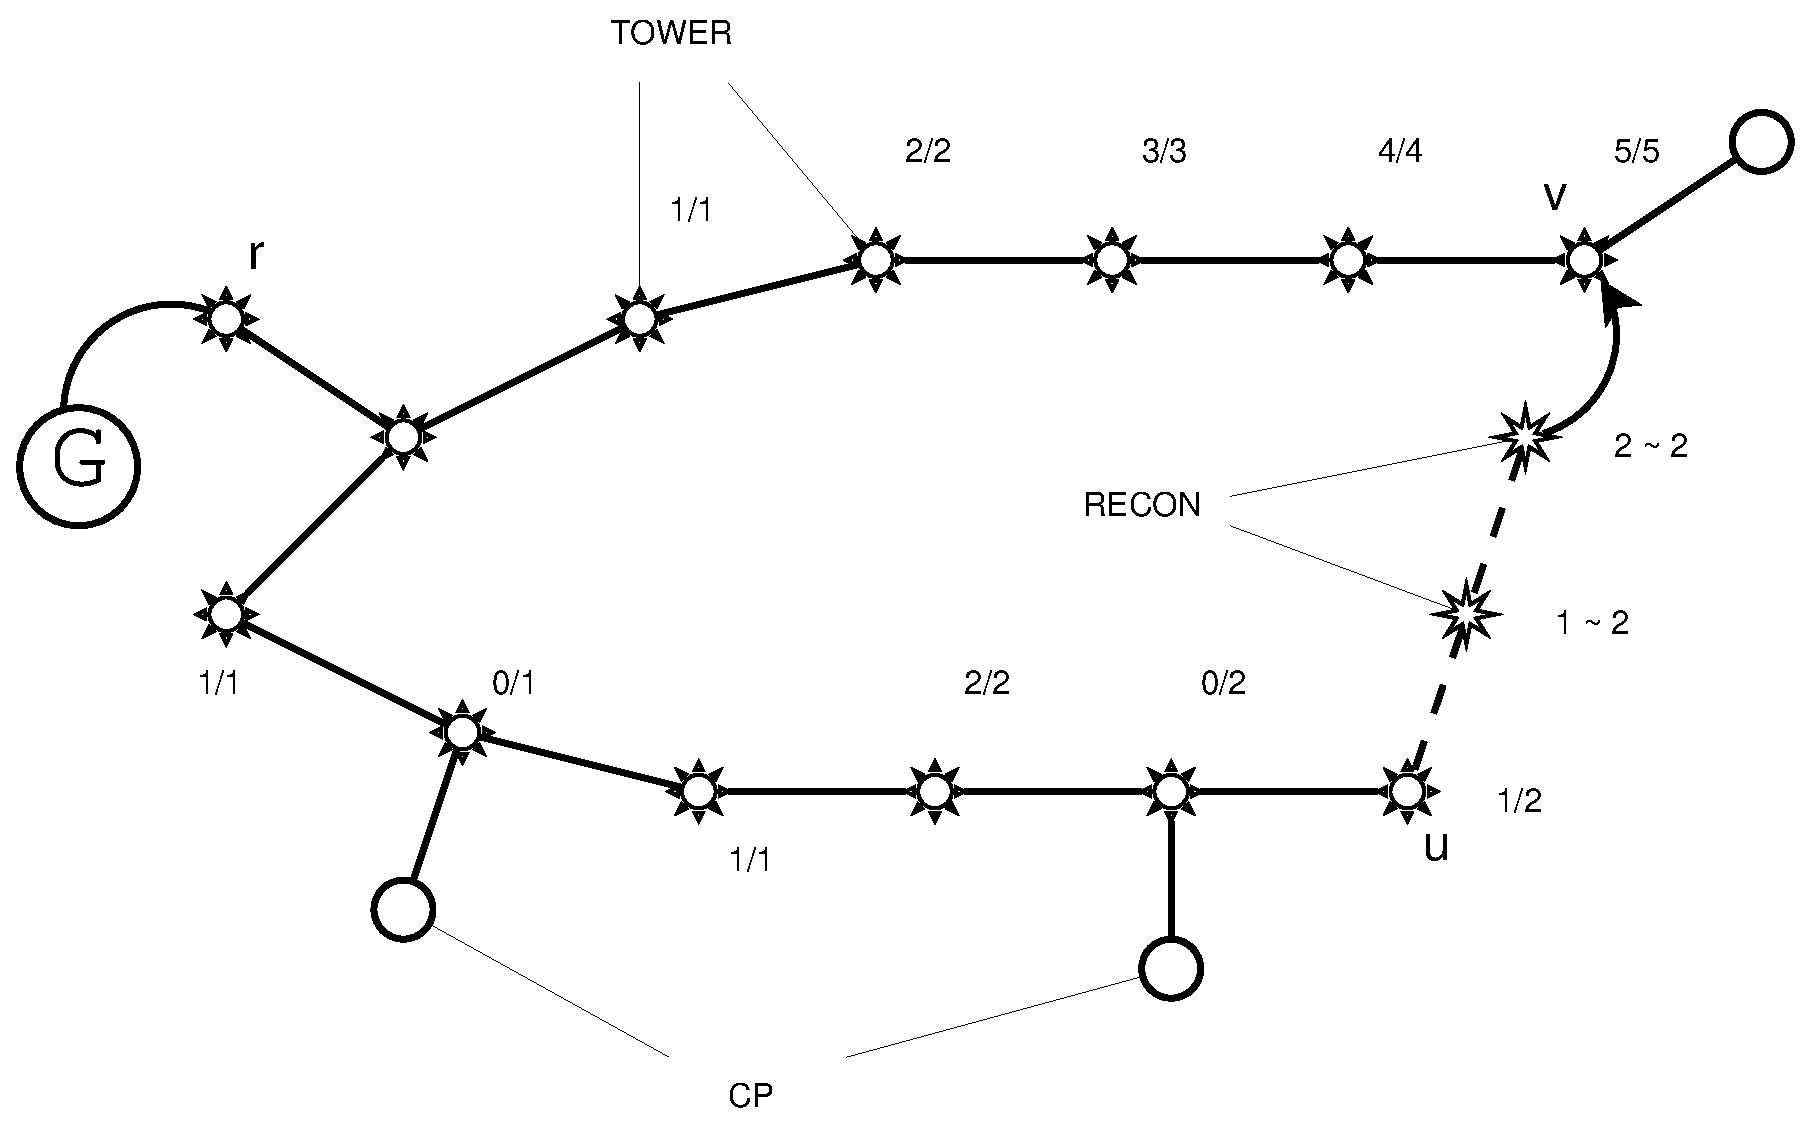
\includegraphics[width=.95\textwidth]{dia/depth_opt}
% \label{fig:comm1}
% \vspace{-1em}
% \caption{m�lys�gi jav�t�s}
% \end{figure}

A \ref{fig:comm1}. �br�n l�that� egy olyan m�lys�gm�r�s, mely eset�ben a t�vols�got az $r$ cs�cst�l m�rt�k �s egy jav�t�sra van lehet�s�g�nk, ugyanis a fels� �g $5$ hossz�, melyet el�rhet�nk egy $3$ hossz�val is. Az �br�n az egyes �gensek mellett felt�ntetett �rt�kp�rok az $l_c/l_m$

Minden $t_d$ id�nk�nt egy el�re megadott kiv�laszt� funkci� meghat�rozza a robotok egy csoportj�t, akikt�l t�vols�got m�r a t�bbi.
A m�r�s elv�gz�se k�zben az al�bbiakat k�zlik egym�ssal:
\begin{itemize}
	\item	$l_c$: jelenlegi hossz\\
			L�ncok hossz�t m�rj�k, �s keress�k az eddig el�fordul� leghosszabbat. Ezt az �rt�ket minden $2$ foksz�m� cs�cs n�veli eggyel, a $3$ foksz�m�ak pedig $0$-ra �ll�tj�k
% z�rt tudatni kell a szomsz�ddal, hogy jelenleg hol j�runk ezt l�p�sr�l l�p�sre n�velik eggyel
	\item	$l_m$: eddigi leghosszabb l�nc, amit tal�ltak\\
			(a leghosszabb l�nc legutols� elemein $l_c=l_m$)
	\item	$l_r$: m�lys�g a kezdem�nyez� cs�cst�l\\
			sz�ks�ges megszabni az ir�ny�t a jav�t�snak, a forr�scs�cst�l k�zelebbivel t�rt�nhet csak jav�t�s
	\item	$i_r$: a m�lys�gm�r�st kezdem�nyez� pont azonos�t�ja\\
	erre az�rt van sz�ks�g, hogy a k�l�nb�z� helyekr�l ind�tott m�r�sek ne keveredhessenek �ssze. Tulajdonk�ppen ez a sz�ne a m�r�snek
\end{itemize}
Folyamat�ban ez a k�vetkez�k�ppen zajlik, ha ilyen m�r�st kap egy cs�cs, akkor az al�bbiak szerint cselekszik:
\begin{itemize}
	\item	ha m�r kapott kor�bban t�vols�gm�r� csomagot, akkor figyelmen k�v�l hagyja
	\item	ha a jelenlegi cs�cs foksz�ma $2$ - vagyis egy egyszer� �sszek�t� cs�cs -, akkor: $l_c=l_c+1$, s ha ez meghaladja az $l_m$-et is, akkor azt is n�veli
	\item	be�ll�tja m�lys�gi sz�l�nek a k�ld�t, �s tov�bbk�ldi minden szomsz�dj�nak, kiv�ve a sz�l�t
\end{itemize}

Teh�t, ha l�tezik olyan �l, amit a gr�fba beh�zva �s t�r�lve  a kialakult k�r legnehezebb �l�t egy k�nnyebbet kapunk, akkor a \ref{fig:comm1}. �br�n l�that� helyzetben:
\begin{equation}
 l_m^u + l_{chain} < l_m^v
\end{equation}
felt�tel teljes�l, �gy jav�t�s v�gezhet�.

\DEF	Steiner-fa:	Adott egy $G=(V,E)$ ir�ny�tatlan, �sszef�gg� gr�f, �s a termin�l pontjainak egy $T$ halmaza ($V$ r�sze), tov�bb� minden �lhez hoz\-z�\-ren\-de\-l�nk egy k�lts�get. Keress�nk egy minim�lis k�lts�g� f�t, amely az �sszes $T$-beli pontot tartalmazza.

\DEF	euklideszi Steiner-fa: $V$ a s�k pontjait tartalmazza
\DEF	maximum $n-2$ darab Steiner-pontot tartalmaz egy $n$ termin�lal rendelkez� fa
\DEF	minden Steiner-pont foka $3$ �s az egyes �lek $120$ fokban indulnak ki bel�le.

\newpage

\XFIG{0.5}{dia/problem_p2}{st00}{Termin�lisok ($T$)}
Legyen $T$ a termin�lis pontok halmaza(\ref{st00}. �bra), melyeket szeretn�nk lefedni egy euklideszi Steiner-f�val.

Ezen pontokra valamilyen m�dszer felhaszn�l�s�val meghat�rozhatjuk a mini\-m�\-lis Steiner-f�t ($S_T$), mely lefedi ezen pontokat (\ref{st01}. �bra).
\XFIG{0.5}{dia/problem_2}{st01}{A $T$-t lefed� $S_T$ Steiner-fa}

% \MEGJ: ilyen esetekben amennyiben ismert a $T$ halmaz a legjobb �ltalam ismert l�tezo algoritmus a GeoSteiner algoritmus \cite{} mely line�ris programoz�s felhaszn�l�s�val oldja meg a feladatot.
% az euklideszi Steiner-fa NP-neh�zs�ge miatt ennek meghat�roz�sa a $T$ halmaz m�ret�t�l f�gg�en 

Mivel a felvetett  probl�ma eset�ben ez a $T$ termin�lishalmaz ak�r meg is v�ltozhat id�vel, ez�rt �rdemes megvizsg�lni azt, hogy mi t�rt�nik, ha m�r ismert egy $T$ termin�lishalmaz Steiner-f�ja, �s ez esetlegesen hogyan viszonyul egy olyan $T'$ termin�lisokat lefed� $S_{T'}$ f�hoz, mely az eredeti $T$ termin�lishalmaznak egy ponttal val� b�v�t�se.
\newpage

Ennek a szeml�ltet�s�hez a kor�bbi f�t b�v�tem egy �j ponttal (\ref{st10}. �bra).

\XFIG{0.5}{dia/problem_2pw}{st10}{Pont hozz�ad�sa}

Amennyiben az �gy l�trej�tt $T'$ termin�lishalmazra �jra megkeress�k az optim�lis Steiner-f�t, abban az esetben a $T'$-h�z tartoz� $S_{T'}$ fa er�sen elt�rhet a $T$ termin�liscsoporthoz tartoz� $S_T$ f�t�l.

Ezt illusztr�lja a \ref{st11}. �br�n l�that� k�k vonalak, melyek az �j fa �lei.

\XFIG{0.5}{dia/problem_2px}{st11}{A $T'$-t lefed� $S_T'$ Steiner-fa}


\MEGJ	Az optim�lis Steiner-fa ilyen m�don val� keres�se ig�nyli a teljes $T$ halmaz ismeret�t. Valamint tov�bbi h�tr�nya, hogy a termin�lis halmaz esetleges v�ltoz�sa eset�n a fa er�sen megv�ltozhat.
% az optim�lis megold�s 'ltoz�sa  felvetett probl�ma megk�veteli hogy a $T$ 

\newpage
% Ezekb�l l�tszik hogy

Egy olyan m�dszer seg�ts�g�vel lenne c�lszer� egy ilyen h�l�zatot fel�p�teni, mely megengedi az iterat�v b�v�t�st, �s fokozatosan k�pes k�zel�teni a Steiner-fa megold�s�t, an�lk�l hogy a fa megszakadna.

A Steiner-fa probl�ma megold�sa megk�zel�thet� heurisztikus algoritmusok se\-g�t\-s�\-g�\-vel, ezek k�z�l kiemeln�m a Steiner Insertion Heuristic nev� \cite{Dreyer98twoheuristics} algoritmust, mely egy picit m�dos�tva egy Steiner-fa b�v�t�v� alak�that� �t.

\xparagraph{steiner\_insertion(T,E)}
\begin{enumerate}
	\item	legk�nnyebb fesz�t�fa megkeres�se a $T$-n
	\item	minden �lre, mely termin�lisokat k�t �ssze $(t_x,t_y)$-ra:
	\begin{enumerate}
		\item	egy olyan $q$ cs�cs keres�se, mely vagy termin�lis vagy Steiner-pont,
			valamint l�tezik a $(q,t_x)$ �l, �s ezen �lek k�z�l a legkisebb sz�get z�rja be a $(t_x,t_y)$ �llel.
		\item	amennyiben a $(q,t_x),(t_x,t_y)$ �lek sz�ge kisebb mint $120$ fok
		\begin{enumerate}
			\item	�j steiner-pont felv�tele ($s$) a $t_x$ poz�ci�j�ba
			\item	�lek elt�vol�t�sa:
			\begin{itemize}
			 		\item	$(q,t_x)$
					\item	$(t_x,t_y)$
			\end{itemize}
			\item	�j �lek felv�tele:
			\begin{itemize}
			 		\item	$(s,q)$
			 		\item	$(s,t_x)$
					\item	$(s,t_y)$
			\end{itemize}
		\end{enumerate}
		\item	lok�lis optimaliz�ci�
	\end{enumerate}
\end{enumerate}

Alapesetben ez az algoritmus egy k�zel�t�st ad a $T$ ponthalmaz Steiner-f�val val� lefed�s�re. Amennyiben �gy m�dos�tjuk hogy csak b�v�tsen egy kor�bbi f�t, akkor azzal m�r �gy k�zel�thetj�k az �j f�t hogy a r�git r�szben megtartjuk.

Egy nagyon nagy el�nye ennek a m�dszernek hogy amennyiben �gy tekint�nk az egyes cs�csokra mint entit�sok, s az �leket mint szomsz�ds�gi kapcsolatokra, akkor a fenti algoritmus bizonyos form�ban lok�lis kommunik�ci�kra alapozva kivitelezhet� az �lek ment�n.

% \newpage
% Az euklideszi Steiner-f�t tekintve a k�vetkez�k igazak:

\DEF
Ha egy $G=(V,E)$ euklideszi Steiner-fa egy $T\subset V$-ra tekintve $\IAO \nexists u,v\in V$ cs�csok, melyek k�z� �let beh�zva a keletkez� k�rnek az $(u,v)$ �le k�nnyebb lenne a k�r b�rmely �l�n�l.

\MEGJ	A t�bbforr�s� m�lys�gm�r�s seg�ts�g�vel a networkers algoritmus ilyen �lek ellen�rz�s�vel igyekszik cs�kkenteni a kialak�tott gr�f s�ly�t.
% t akkor az ezzel alkotott k�r ne lenne a legnehezebb �le a k�rnek.

% \BIZ	
% \FWD \\ha $G$ Steiner fa akkor a legk�nnyebb fa ami a benne foglalt pontokat �sszek�ti\\
% \BWD sajnos ez m�g nem stimmel...120 fok?, $|S|\leq|T|-2$, 

% \DEF	kb:egy Steiner f�ban a bels� melyben a bels� cs�csok foksz�ma $3$ - azok a szomsz�dait 120 fokos sz�gben l�tj�k.

% \xparagraph{Kapcsolatok a Steiner f�val}
% \sout{
% Amennyiben siker�l a fentiek alapj�n folyamatosan jav�tani a h�l�zaton, �gy bizonyos m�rt�kben megk�zel�thet� a pontok Steiner f�val val� lefed�se. Ezt a k�pess�get jelenleg m�g teljes m�rt�kben nem siker�lt be�p�teni, amennyiben k�t torony egym�s kommunik�ci�s k�rnyezet�be �r elv�gzik a meg\-fe\-le\-l� �lek cser�j�t. A felder�t�kre val� kiterjeszt�s�t m�g nem fejeztem be.
% Steiner f�t lehets�ges �s aj�nlott is approxim�ci�s algoritmusokkal k�zel�teni, a fenti m�dszer kialak�t�s�hoz sokat seg�t Dreyer �s Overton cikke a Steiner-f�t k�zel�t� heurisztik�kr�l (\cite{Dreyer98twoheuristics},).
% % A tornyok �ltal haszn�lt er�k, melyek haszn�latban vannak az optimaliz�ci� els� r�sz�ben olyanok, amiknek a nyugalmi �llapota a $0$ t�vols�gon van. Ez�rt a robotok ebben az �llapotban az �ket k�r�lvev�k �ltal meghat�rozott s�kidom s�lypontj�ba prob�lnak �llni. Ha $2$ szomsz�dja van, akkor egy egyenesre �ll vel�k, ha $3$ szomsz�dja van, akkor a h�romsz�gnek a s�lypontj�ba, ami ismert, hogy s�lypontb�l az egyes cs�csok $120$ fokot bez�r�an l�tszanak.\\
% % Rem�nyeim szerint az algoritmus valamilyen k�zel�t�ssel egy Steiner f�t prob�l megtal�lni. A k�zel�t�s m�rt�ke a radart�vols�t�l f�gghet valamilyen m�rt�kben.
% }
\newpage


\subsubsection{Priorit�s}

\hspace{2em}Az �genseknek sz�ks�ge van egyfajta id�r�l id�re t�rt�n� kit�ntet�sre, p�ld�ul egy kapcsolat megsz�ntet�se �s annak helyettes�t�se egy m�sikkal egy �gens sz�m�ra megengedett kell legyen, de amennyiben t�bb �gens is egyszerre ``gondolja\phantom{}'' ezt, akkor az z�rzavart okozhat.

A priorit�s bevezet�s�re csak lok�lisan van sz�ks�g, ugyanis egy torony eset�ben el�gs�ges, ha a szomsz�daihoz m�rten van priorit�sa.

% T�bb helyen gondot okozhatna egyidej� d�nt�shozatal ez�rt sz�ks�ges volt egy megold�s bevezete

El�ny�s lenne, ha nagyon gyakran ker�lne �jra �s �jra priorit�sba minden cs�cs �s a legjobb lenne, ha nem kellene hozz� kommunik�ci�. Ez�rt a sorozatsz�mok, valamint az eltelt id� seg�ts�g�vel kell kisz�molni egy logikai �rt�ket.

A priorit�s f�ggv�nnyel szemben azonban t�masztanunk kell egy megk�t�st - nem lehet k�t szomsz�d egyszerre priorit�sban:
\DEF	Adott egy $G=(V,E)$ gr�f, �s egy $\varphi : V \TO \setL
% \footnote{$\setL = \{true,false\}$ logikai �rt�kek}
$.
A $\varphi$ egy megengedett prioriz�l�sa a cs�csoknak amennyiben:
% $$ \forall v \in V : \varphi(v) : \nexists u \in V : \varphi(u) \AND (u,v) \in E $$
\begin{equation}
\nexists (u,v) \in E : \varphi(v) \AND \varphi(u)
\end{equation}

A feladat a k�vetkez�k�nt fogalmazhat� meg:
\FEL	Adott egy tetsz�leges gr�f, melynek foksz�m�ra ismer�nk fels� kor\-l�\-tot. Va\-lamint adott $2^s$ fels� korl�t a cs�csok sz�m�ra �s adottak a $\tau=\{\varphi_1,...,\varphi_n\}$ prioriz�l�sok, amennyiben
$\forall u \in V : \exists i\in[1:n] : \varphi_i(u)$ teljes�l tet\-sz�\-le\-ges $k$ foksz�m korl�tos gr�f eset�n, melynek legfeljebb $2^s$ cs�csa van, akkor $\tau$ megold�sa a gr�f szabad priorit�s�nak.

% A probl�m�t megk�zel�thetj�k �gyis, hogy feltessz�k, hogy egy szob�ban $s$ darab izz� van. Bemegy egy ember $k$ darab cetlivel melyekre tetsz�legesen fel�rhatja hogy f�nyes vagy s�t�t. Hogy kapcsoljuk az izzokat hogy a leheto legkevesebb l�p�s ut�n a cetliknek megfelel�en vil�g�tsanak az izz�k?
% 
% Egy m�sik �tfogalmaz�sban ugyanez a probl�ma: Vegy�nk egy $s$ dimenzi�s hiperkock�t, h�ny cs�csot kell kiv�lasztani bel�le hogy minden cs�cs�t lefedj�k $s-k$ t�vols�gon bel�l?

% \xparagraph{alternat�v feladat} vegy�nk egy $l$ hosszu bin�ris sorozatot, s ennek $s$ hossz� r�szsorozatait $x_i,..x_{i+s-1}$ - ...

% \MEGO a $k=3$ esetre
% vegy�nk egy r�szhalmaz�t a term�szetes sz�moknak legyen ez $S$.
% legyen $l=\ceil{\log_2{\max{S}}}$.
% \begin{align}
% \forall a,b,c \in S : a\neq b \AND a\neq c : \exists t \in \setN :\\
% \varphi_t^l(a) > \varphi_t^l(b) \AND \varphi_t^l(b) < \varphi_t^l(c) 
% \end{align}
% 
% % \OTLET nezzunk binaris szamokat es figyeljuk meg az elso pontot ahol eloszor k�l�nbs�gek vannak a h�rom sza
% 
% a tulajdons�gnak megfelel� f�ggv�ny:
% 
% $\varphi(x,i,l)=\left\{\begin{array}{lr}
% x\Xor (2^i-1)				&	\mbox{ha } i<=l\\
% \varphi(x,i-l,l)\Xor (2^l-1)	&	\mbox{k�l�nben}
% \end{array}\right.$\\
% a fenti k�pletben: $\varphi_t^l(x)=\varphi(x,t,l)$
% \MEGJ	ez kb olyan mintha 1-1 neg�ci�s vihar szaladna �t a sz�mokon.
% el�sz�r v�gigneg�lja el�sz�r csak az els�t azt�n egyre t�bbet, s amikor el�ri a v�g�t ugyan�gy veszi le is ;)
% 
% \BIZ	legyen: $a,b,c \in S$, rendezz�k a sz�mokat mondjuk $a>b>c$,
% ebben az �llapotban a $c$ a legkisebb ez�rt az m�r teljes�l is.
% Ha minden sz�mot neg�lunk akkor a $a<b<c$ is teljes�l. $\TO a$-val is k�sz vagyunk.
% vegy�k azt az $i$. bitet melyen eld�lt hogy $b>c$, ezt, �s az enn�l kisebb helyi�rt�k� biteket neg�lva m�r a tulajdons�g megfordul. Ez�rt ez $k=3$-ra megold�s.


% \xparagraph{``Kiz�r� vagy'' m�velet felhasz�l�sa erre a c�lra}
% Adott $k+1$ darab sz�m: $x^1,x^2,...,x^k$ valamint $y$, ezek k�z�l szeretn�nk bel�tni hogy l�tezik olyan $z$ sz�m mely eset�n:
% \newcommand{\XOR}{\otimes}
% $$ z\XOR y < z \XOR x_i : \forall i \in [1:k]$$
% l�tezik $t_1,t_2,...,t_k$ eg�sz sz�mok melyekkel ahol $y$ �s $x_i$ el�sz�r t�rnek el. Amennyiben ezt a


\xparagraph{C�mk�z�s}
Vegy�nk egy tetsz�leges $k$ foksz�m korl�tos egyszer� gr�fot($G(V,E)$), �s egy olyan c�mk�z�s�t a cs�csoknak, mely minden cs�cshoz k�l�nb�z� sz�mokat rendel a $\setN$ halmazb�l.


Ir�ny�tsuk meg a gr�f �leit a c�mk�z�s szerint �rtelmezet '$<$' rel�ci� seg�ts�g�vel.\\
�rtelmezz�k a gr�f $x,y$ cs�csaira a k�vetkez� f�ggv�nyt:
\begin{align}
 t(x,y)=\Floor{\log_2 ( s(x) \Xor s(y) ) }
\end{align}
C�mk�zz�k fel az �leket a k�vetkez� m�don:
az $(x,y)\in E$ �lhez rendelj�k a $t(x,y)$ f�ggv�ny �rt�k�t:
$b_{x,y}=t(x,y)$.

% C�mk�zz�k fel a gr�f �leit a $t$ f�ggv�ny seg�ts�g�vel.
A $t(x,y)$ f�ggv�ny megmondja hogy a c�mk�z�s h�nyadik bitj�nek neg�l�sa ford�tan� meg az $x$ �s $y$ cs�csok k�z�tti '$<$' rel�ci�t.

Vegy�k az �gy elk�sz�tett gr�f egy $u$ cs�cs�t �s vizsg�ljuk meg a szomsz�dait ($N(u)=\{ v_1,v_2,..,v_r\}$).

% \newpage


 \XFIGG{0.9}{dia/fp_1}{fp_1}{Az $u$ cs�cs �s szomsz�dai}{
  \psfrag{N_1}[cc][lb]{$v_1$}
  \psfrag{N_2}[cc][lb]{$v_2$}
%   \psfrag{N_k1}[cc][lb]{$n_{k-1}$}
  \psfrag{N_k}[cc][lb]{$v_r$}
  \psfrag{N_i}[cc][lb]{$v_i$}
  \psfrag{N_j}[cc][lb]{$v_j$}
  \psfrag{1}[lb][lb]{$b_1$}
  \psfrag{2}[lb][lb]{$b_2$}
  \psfrag{i}[lb][lb]{$b_i$}
  \psfrag{j}[lb][lb]{$b_j$}
  \psfrag{k}[lb][lb]{$b_r$}
  \psfrag{U}[cc][lb]{$u$}
 }

Az elk�sz�tett gr�f �s az �lek c�mk�z�se l�that� a \ref{fp_1}. �br�n.
\ALL
Amennyiben $u$ k�t k�l�nb�z� szomsz�dj�val ($v_i,v_j$)  �sszek�t�   �lekre ugyanazon ($b_i=b_j$) c�mke ker�lt, akkor ezen k�t �l nem alkothat utat a $v_i,v_j$ cs�csok k�z�tt.
\BIZ
Az �lek c�mk�z�se a legnagyobb ($z.$) bitet jel�li, melynek neg�l�sa eset�n a k�zt�k fenn�ll� '$<$' rel�ci� megfordul.
Az $u,v_i,v_j$ cs�csokon k�v�l dobjuk el a gr�f �sszes t�bbi pontj�t.
�s a cs�csok c�mk�z�s�t sz�k�ts�k le a $z.$ bitre. Mivel az $u,v_i,v_j$ csak ett�l f�gg�tt, ez�rt a k�zt�k fut� �lek ir�nya �s c�mk�je az eredetivel megegyez� marad. A lesz�k�t�s miatt viszont m�r csak k�t �rt�ket tartalmaz a cs�csokhoz rendelhet� c�mk�k halmaza, de �gy biztosan nem alakulhat ki h�rom hossz� ir�ny�tott �t.

\ALL
V�lasszunk egy $(u,v_i)$ �let, �s egy tetsz�leges $r\in \setN$ sz�mot.
Ekkor, az $s'(x)=s(x) \Xor 2^r$ �jrac�mk�z�s eset�n az $(u,v_i)$-�l ir�ny�t�sa akkor �s csak akkor fordul meg ha $r$ megegyezik az �l c�mk�j�vel $z$, vagyis ha $z=r$ teljes�l.
% Amennyiben az $(u,v_i)$ �l $z$-vel van c�mk�zve, egy $s'$ c�mk�z�s eset�n, melyet �gy kaptunk hogy: $s'(x)=s(x) \Xor 2^r$, akkor �s csak akkor fordul meg az �j c�mk�z�sben megkonstru�lt gr�fban ez az �l amennyiben $z=r$.
\BIZ
\begin{itemize}
 \item 
$r>z$ eset�ben az $s(u)$ �s $s(v_i)$ sz�mok $r.$ bitje meg kellett hogy egyezzen, ez�rt a neg�l�sa nem v�ltoztat a k�zt�k fenn�ll� rel�ci�n.
\item
	$r<z$ eset�ben mivel a $z.$ bit nagyobb helyi�rt�ket foglal el, ez�rt a rel�ci� erre �rz�ketlen marad.
\item	$r=z$	eset�ben megfordul a rel�ci�.
\end{itemize}

\xparagraph{K�vetkezm�ny}
K�sz�ts�nk el egy sz�mot az $u$-b�l ki/befut� �lek c�mk�z�se �s ir�nya alapj�n. A kifut� �lekre �rt c�mk�ket gy�jts�k a $G$ halmazba, a befut�kat pedig az $L$ halmazba. Vegy�nk egy olyan sz�mot($w$) melynek $G$ halmazba tartoz� bitjei $0$-�k, �s minden $L$ halmazba tartoz� bitje $1$.
Mivel $G \Inter L=\emptyset$, ez�rt ilyen sz�m l�tezik.

Vegy�k az $s'(x)=s(x) \Xor w$ c�mk�z�st, ebben az esetben az $u$ cs�csnak csak kifut� �lei lesznek.

% Nem l�tezik $v_i,v_j$ szomsz�d melyek $(u,v_i)$ �s $(u,v_j)$ �lei ugyanazon sz�mmal lettek c�mk�zve

Egy olyan �tc�mk�z�re van sz�ks�g, mely k�pes v�letlenszer�en cs�csokat ki\-t�n\-tet\-ni. A fentiek alapj�n minden cs�cs rendelkezik valah�ny bitre val� el��r�ssal annak kit�ntet�s�hez - viszont a t�bbi bitre nincs kik�t�se.

\xparagraph{Megold�s: v�letlen}

A fenti felt�teleket egy v�letlensz�mgener�tor teljes�ti, ugyanis abban tet\-sz�\-le\-ge\-sen t�vol �ll� bitek mintav�telez�se eset�n  egyenletes eloszl�st kapunk \cite{COMPLEX}. �gy a priorit�sok meg�llap�t�sa t�rt�nhet egy olyan pszeudo v�\-let\-len\-sz�m\-ge\-ner\-�\-tor\-ral, mellyel minden k�rben az �sszes �gensen ugyanazt a v�letlen sz�mot �ll�tja el�, �s ezzel a v�letlensz�mmal bitenk�nti kiz�r� vagyot haszn�lva �jrac�mk�zz�k az �sszes cs�csot, melyek az �gy �tc�mk�zett gr�fban minden szomsz�djukn�l kisebbek lesznek priorit�sban.

\newpage	

\subsubsection{Kommunik�ci�s minta}

Amennyiben a torony szerepet bet�lt� robotok �zeneteire nem teszek meg\-k�\-t�st, akkor megt�rhet a fa jellege a ki�p�tett h�l�zatnak, ez�rt a networkerek a kommunik�ci�jukat az al�bbi szab�lyok alapj�n v�gzik:


% k�t k�l�nb�z� m�dszerrel �zennek egym�snak,
% %  mivel a kett� f�ggetlen alkalmaz�sa megt�rn� az alakul� gr�f fa tulajdons�g�t. Ez�rt a k�vetkez� kommunik�ci�s szab�lyokkal m�k�dnek:
\begin{itemize}
	\item	minden robot $3$ id�egys�gre kap priorit�st
	\item	ha egy cs�cs foksz�ma $1$-re cs�kken - kiv�lhat a gr�fb�l, ha
% 		\begin{itemize}
% 			\item	
van priorit�sa a l�p�s $0.$ f�zis�ban.
% 		\end{itemize}
	\item	\LI -t csak akkor k�ldhet egy torony, ha
% 		\begin{itemize}
% 			\item	
van priorit�sa
% 			\item	
a l�p�s $0.$ f�zis�ban
% 		\end{itemize}
	\item	\SI -t csak akkor k�ldhet, ha
% 		\begin{itemize}
% 			\item	
van priorit�sa
% 			\item	
a l�p�s $1.$ f�zis�ban
% 		\end{itemize}
\end{itemize}
% ez a szab�lyrendsz

\begin{figure}[h]
\vspace{-1em}
% \centering
% \includegraphics[width=.94\textwidth]{dia/fuelpump_slowdown}
% \hspace{-5em}
\centering
\psfrag{SUBJ}[lt][lt]{`` t�ma ''}
\psfrag{LINKI}[lt][lt]{{\LI}}
\psfrag{SI}[lt][lt]{{\SI}}
\psfrag{IL}[lt][lt]{{\IL}}
\psfrag{LE}[lt][lt]{{\LE}}
\includegraphics[width=.55\textwidth]{dia/comm1_3step}
\vspace{-2em}
\caption{$\TOWER$ comm}
\label{asd1}
% 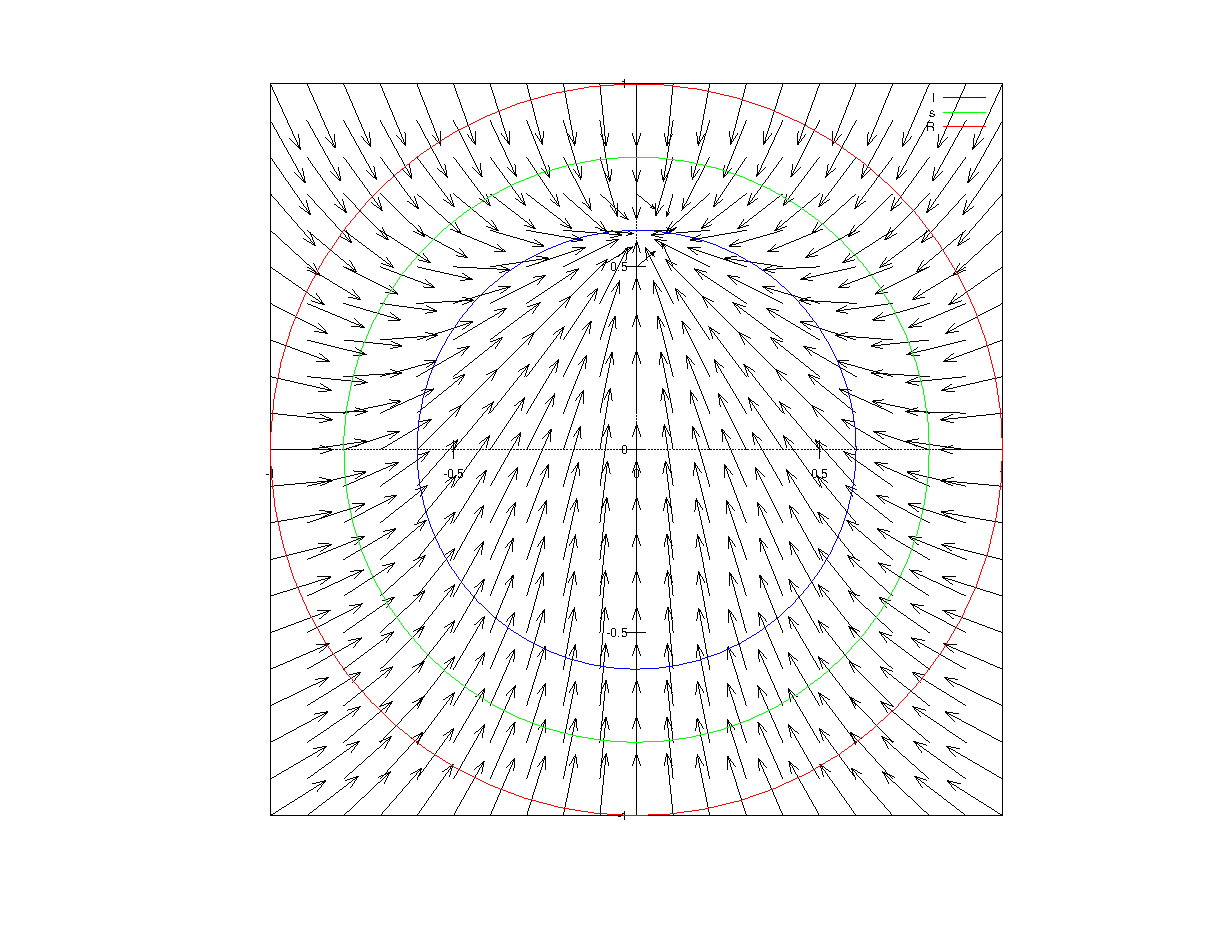
\includegraphics[width=0.55\textwidth]{fig/scan_repos}
% \vspace{-5em}
\end{figure}

Az �gy kialakul� kommunik�ci�s minta \ref{asd1}. �br�n l�that�, melyen a k�vetkez�k t�rt�nnek:
\begin{itemize}
	\item a $r$ cs�cs kiv�lik a gr�fb�l, s az $1$-es f�zisban m�r keres�v� is v�lik.
	\item	a $b$ cs�csnak megvan a priorit�sa a k�rre, ez�rt t�j�koztatja $c$-t az $a$ jel� szomsz�dj�r�l $|c-a| < d_{r}$
	\item	az $1.$ f�zis kezdet�n $c$ eld�nt�tte, hogy kiv�n �lni a lehet�s�ggel �s �tveszi $b$-t�l az $a$ cs�csot, ez�rt bontja a kapcsolat�t $b$-vel �s jelzi $a$-nak, hogy van egy �j szomsz�dja
	\item	ek�zben $b$ elk�ldi $u$-nak, akit l�t ugyan, de mivel nem ismeri, ez�rt t�j�koztatja arr�l, hogy a legutols� t�vols�g m�r�sben mennyire is volt � t�vol.
	\item	az $u$ cs�csnak tetszik az aj�nlat - k�nnyebb� v�lik a gr�f ha � $b$-vel van �sszek�tve,
		ez�rt bontja a kapcsolat�t a m�lys�gi sz�l�j�vel, �s visszajelez $b$-nek, hogy helyre�lljon a szimmetria
\end{itemize}

\BIZ
Ha ez a kommunik�ci�s minta hib�hoz vezetne, az k�tf�lek�pp k�pzelhet� el:
\begin{itemize}
	\item	k�t komponensre szakad a gr�f
	\item	kialakul egy k�r
\end{itemize}
mivel mindk�t esetben a $|E|=|V|-1$ felt�tel s�r�l, ez�rt csak a k�vetkez�t kell bel�tni:
nem fordulhat el� az, hogy k�t cs�cs ugyanarr�l az �lr�l nyilatkozik egym�snak k�l�nb�z� d�nt�seket:
\begin{itemize}
	\item 
	a $0.$ k�rben csak \LE\ elk�ld�s�re ker�lhet sor, mely ha a m�sik oldalr�l is \LE, akkor �ppen megsz�nik a gr�funk, ami a vezet� megl�te miatt elk�pzelhetetlen.
	Valamint, mivel jelenleg $r$ priorit�sban van, ez�rt $r$ egyetlen �le sem sz�nhet meg, ugyanis a szomsz�dai biztosan nincsenek priorit�sban.
	\item	az $1.$ k�rben elhangz� �zenetek kiz�r�lag a $b$ cs�cs kommunik�ci� k�rnyezet�ben lev� �lekre vonatkozik, ez�rt biztosan csak maximum egy cs�cs fog nyilatkozni k�t �lr�l
	\item	a $2.$ k�rben: ha az $1.$ k�rben t�rt�nt esem�nyek miatt v�ltozott a fel�ll�s az $u$ cs�cs sz�m�ra �s m�r nincs �sszek�tve a m�lys�gi sz�l�j�vel, akkor figyelmen k�v�l kell hagynia az �zenetet (ha t�bbet kap, akkor is csak eggyel foglalkozik), �s mivel a m�lys�gi sz�l�j�nek � nem lehet sz�l�je, ez�rt ott nem lehet �zenet duplaz�s. Mivel $u$ eddig nem volt �sszek�tve $b$-vel, ez�rt annak a kapcsolatnak a l�trehoz�sa semmilyen akad�lyba nem �tk�zhet.
\end{itemize}

\newpage
\input{parts/70_tower_algo}
\input{parts/95_open_issues}


%----------

% \input{parts/A0_conclusion}
% \xparagraph{open issuies--------}
% 
\subsection{Alternat�v�k}



\b{ez a szekci� val�szin�leg kimarad - mert m�g mind�g kidolgoz�s alatt �ll --> nem teljes/m�g nincs alkalmazva, a cs�nya er�teres j�t�kot ejti ki}




R�gz�ts�nk egy $\alpha$ param�tert mely az egyes l�p�sekben val� ir�nyv�ltoztat�s maximuma.\\
Legyen $\vec{t_{i}^t}$ az $i.$ cs�cs $t.$ id�pillanat�ban haszn�lt ir�nyvektora.\\
A fenti $\alpha$ korl�toz�s a k�vetkez�ket eredm�nyezi:\\
$\vec{d_{i}^t}\vec{d_{i}^{t+1}} \le \sin \alpha  $\\
valamint mivel a szomsz�doknak a saj�t ir�nyvektor�t k�zvet�ti ez�rt igaz lesz a k�vetkez� is:\\
$\vec{d_{i}^t}\vec{d_{i+1}^{t}} \le \sin \alpha  $\\
$\vec{d_{i}^t}\vec{d_{i-1}^{t}} \le \sin \alpha  $\\

\newpage
\subsection{A hib�z�s b�ntet�f�ggv�nye}

\begin{wrapfigure}{R}{0.33\textwidth}
\vspace{-2em}
\psfrag{EMIN}[lb][lb]{$e_{min}$}
\psfrag{EMAX}[lb][lb]{$e_{max}$}
\psfrag{E}[lb][lb]{$e$}
\psfrag{G}[lt][lt]{$G$}
\psfrag{S}[lt][lt]{$s$}
\psfrag{P0}[lt][lt]{$P$}
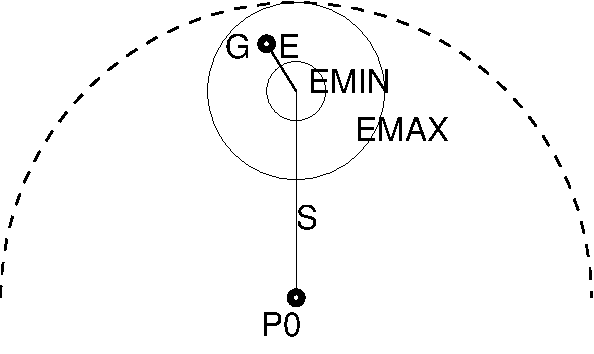
\includegraphics[width=.33\textwidth]{dia/scan_errors}
% 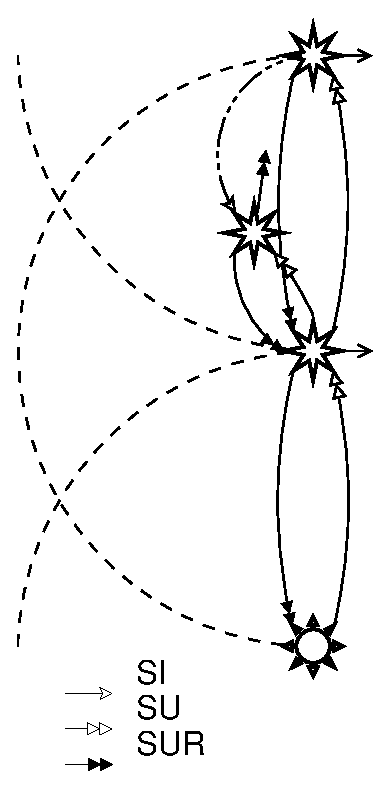
\includegraphics[width=.13\textwidth]{dia/scan_merge}
% \caption{�zenetek keres�s k�zben}
\vspace{-2em}
\label{ref:merge}
\end{wrapfigure}

Amennyiben be lehet vezetni egy olyan b�ntet�f�ggv�nyt ami akkor kedvez a legjobban a el�rehalad�snak ha az minim�lis, viszont alacsonyan tart�s��rt a szomsz�d �gens a felel�s akkor az automatikusan �letbe fog l�pni ha a l�nc v�ge nem tudja tartani a temp�t.\\
R�gz�ts�nk egy keres�t az orig�ban, melynek a keres�si ir�nya legyen az $(1,0)$ vektor, �gy felvehet�nk egy $D=(0,s)$ pontot ami az el�nyben r�szes�tett poz�ci� lesz.\\



asdasddas
asdasddas
asdasddas
asdasddas\\
asdasddas
asdasddas
asdasddas
asdasddas\\
asdasddas
asdasddas
asdasddas
asdasddas\\
asdasddas
asdasddas
asdasddas
asdasddas\\
asdasddas
asdasddas
asdasddas



\subsection{Legrosszabb eset}


\begin{wrapfigure}{L}{0.33\textwidth}
\vspace{-2em}
\psfrag{EMIN}[lb][lb]{$e_{min}$}
\psfrag{EMAX}[lb][lb]{$e_{max}$}
\psfrag{E}[lb][lb]{$e$}
\psfrag{G}[lt][lt]{$G$}
\psfrag{S}[lt][lt]{$s$}
\psfrag{P0}[lt][lt]{$P$}
\includegraphics[width=.33\textwidth]{dia/scan_worst_case}
\vspace{-2em}
\label{ref:merge}
\end{wrapfigure}



%Egy �gens maxim�lisan $v_{max}$ sebess�ggel mozoghat ez�rt

A keres�s folyam�n a l�nc m�rete alapj�n egy cs�cs maximum $\frac{k}{l}$ sebess�ggel mozoghat, ahol $l$ a teljes l�nc hossza, �s $k$ pedig a sz�ban forg� robot t�vols�ga a kiindulas'ipontt�l.
A fenti mozgat� f�ggv�nynek ez alapj�n az al�bbiakat kell teljes�tenie:
tegy�k fel a legrosszabbat a keres�nk kics�szott az ismert t�l m�rt $1$ sugar� k�rre.
Vegy�k ezt az elemet a $k.$-nak az $l$ hossz� l�ncban. �s tegy�k fel azt is hogy a $k-1$ - az ismer�se is kics�szot, �s a lehet� legrosszabb ir�nyba l�p tov�bb,
de mivel a $k-1$. cs�cs csak maxim�lisan $\frac{k-1}{l}$ sebess�ggel mozdulhat el, ez�rt ha az $f$ f�ggv�ny $1$ sugar� kor�n a vektorok t�k�letesen befele mutatn�nak akkor soha nem fordulhatna el� az hogy egy cs�cs leszakad a keres�k k�zul.\\
Ennek a tulajdons�gnak az ellen�rz�s�re haszn�lhat� az al�bbi m�dszer:
	vegy�k a k�vetkez� f�ggv�nyt:
\begin{align*}
		w_x(x,y)&=-x \\
		w_y(x,y)&=-y
\end{align*}
�s amennyiben $\forall (x,y) \in \setR : x^2+y^2 \le 1 : f(x,y)+\frac{w(x,y)}{|w(x,y)|} > 0 $, akkor ez tulajdons�g teljes�l - �s akkor egy megengedett �llapotb�l kiindulva soha nem veszhet el elem.



K�l�n-k�l�n vizsg�lva az egy pont k�r�li k�rmozg�st �s az egyenes ir�nyba val� elmozdul�st



ir�nyvektor:	$\vec{t}$\\
$\vec{t}$\\
$ G = P + (0,s) $\\
$ P=(0,0)$\\
$ \vec{t}=(1,0) $\\
$ P'= v_{max} ( \cos\alpha, -\sin\alpha)  $\\
$ d=|P'-G| < 1$\\
$ |P'-G|^2 < 1$\\
% $ v_{max}^2 \cos\alpha^2 + $\\
$ |(v_{max} \cos\alpha, s+v_{max} \sin\alpha)|^2 < 1 $\\
$ s^2+2s v_{max}\sin\alpha +v_{max}^2-1 < 0 $\\
$ s = v_{max}\sin\alpha+\frac{\sqrt{4\sin^2\alpha - 4 (v_{max}^2-1)}}{2}$\\
$ s = v_{max}\sin\alpha+\sqrt{\sin^2\alpha -  (v_{max}^2-1)}$\\
$ s = v_{max}\sin\alpha+\sqrt{1+\sin^2\alpha - v_{max}^2}$



% \cite{PA}
\renewcommand*{\refname}{} % This will define heading of bibliography to be empty, so you can...
\section{Irodalomjegyz�k}  

\bibliographystyle{plain}	% (uses file "plain.bst")
\bibliography{bibtex}		% expects file "myrefs.bib"
% \bibliography{}		% expects file "myrefs.bib"


% \section{Szimul�ci�s k�rnyezet}
% Az algoritmust futtat� szimul�ci�s rendszer erre a c�lra lett k�sz�tve, a megjelen�t�shez/m�k�d�shez OpenGL-re �s 


% \begin{center}
% Network building and maintenance is the foundation of today's information exchange methods -
% but in a hostile or evolving environment it can be hard to maintain a network with the classical methods.
% This papers aim is to explore the possibilities, problems and options how the global network could be handled locally.
% \sout{cooperative network building from local informations\\
% kooperativ robotok h�l�zat�p�t�sre}
% \end{center}

% \newcommand{\cp}{\complement}




\end{document}

